\documentclass[polish]{article}


\usepackage{blindtext}
\usepackage{amsmath}
\usepackage[utf8]{inputenc}
\usepackage[polish]{babel}
\usepackage[T1]{fontenc}
\usepackage{listings}
\usepackage{color}
\usepackage{amssymb}
\usepackage{esvect}
\usepackage{graphicx}
\usepackage{caption}
\usepackage{hyperref}
\usepackage{float}
\usepackage{siunitx}

\usepackage{etoolbox}
\patchcmd{\thebibliography}{\section*{\refname}}{}{}{}

\graphicspath{ {./obrazy/} }

\definecolor{dkgreen}{rgb}{0,0.6,0}
\definecolor{gray}{rgb}{0.5,0.5,0.5}
\definecolor{mauve}{rgb}{0.58,0,0.82}

\lstset{frame=tb,
  language=Python,
  aboveskip=3mm,
  belowskip=3mm,
  showstringspaces=false,
  columns=flexible,
  basicstyle={\small\ttfamily},
  numbers=none,
  numberstyle=\tiny\color{gray},
  keywordstyle=\color{blue},
  commentstyle=\color{dkgreen},
  stringstyle=\color{mauve},
  breaklines=true,
  breakatwhitespace=true,
  tabsize=3
}

\newcommand*{\captionsource}[2]{%
  \caption[{#1}]{%
    #1%
    \\\hspace{\linewidth}%
    \textbf{Źródło:} #2%
  }%
}

\title{Wykrywanie wdechu i wydechu na podstawie dźwięku z mikrofonu}
\author{Dominik Lau, Mateusz Kowalczyk, Michał Tarnacki}



\begin{document}

\maketitle

\section{Wstęp}
Celem projektu było określanie chwil na nagraniu, w których osoba bierze wdech i wydech. 
Dokonano oceny jakościowej za pomocą detekcji oddechu na żywo jak i ilościowej (przy wykorzystaniu
dalej wymienionej metryk).

\section{Teoria}
\subsection{Dyskretna transformata Fouriera (DFT)}
W celu przejścia z dziedziny natężenia od czasu do dziedziny częstotliwości stosujemy dyskretną transformatę
Fouriera.  DFT przekształca ciąg skończonych próbek sygnału $a_0, a_1, a_2, ..., a_{N-1}$ w ciąg 
$A_1, ..., A_{N-1} \in \mathbb{C}$
\begin{gather*}
	A_k = \Sigma_{n=0}^{N-1} a_ne^{\frac{-kni\pi}{N}}, 0 \le k \le N-1
\end{gather*}
W naszych zastosowaniach będziemy brali pod uwagę tylko część rzeczywistą tego wielomianu
\begin{gather*}
	R_k = Re(A_k), 0 \le k \le N-1
\end{gather*}
Skorzystamy z odmiany dyskretnej transformaty Fouriera - STFT (krótkoczasowa transformata Fouriera). 
Jest to zadaniczo transformacja Fouriera jednak wykonywana w mniejszych oknach czasowych. Dzięki temu otrzymujemy informację o zmianie widma w czasie, czyli jednocześnie posiadamy informację o właściwościach zarówno w dziedzinie czasu jak i częstotliwości. Najistotniejszym parametrem tej metody jest rozmiar okna. Ponieważ iloczyn jego szerokości w dziedzinie czasu i szerokości w dziedzinie częstotliwości jest stały dla danego okna, poprawiając rozdzielczość czasu, pogarszamy rozdzielczość częstotliwości.
Naszą funkcję natężenia w czasie dla pewnego okresu $t \in [t_0, t_0 + B]$, gdzie $B$ - rozmiar okna (przyjmujemy $B=1024\approx \frac{1}{44} s$) przedstawiamy zatem jako 
\begin{gather*}
	I(t) = \Sigma_{f} I_{f}(t)sin(2 \pi f t)
\end{gather*}
stąd dla danego przedziału w czasie jesteśmy w stanie stworzyć wektor natężeń
\begin{gather*}
	\boldsymbol{I} = [I_{f_1}, I_{f_2}, ..., I_{f_n}]
\end{gather*}
W dalszych rozważaniach wykorzystujemy także średnią częstotliwość, którą liczymy ze wzoru
\begin{gather*}
	\bar{f} = \frac{\Sigma_ffI_f}{I}
\end{gather*}
Wykorzystujemy implementację transformaty z biblioteki $numpy$ oraz $tensorflow$.
\begin{figure}[H]
	\centering
	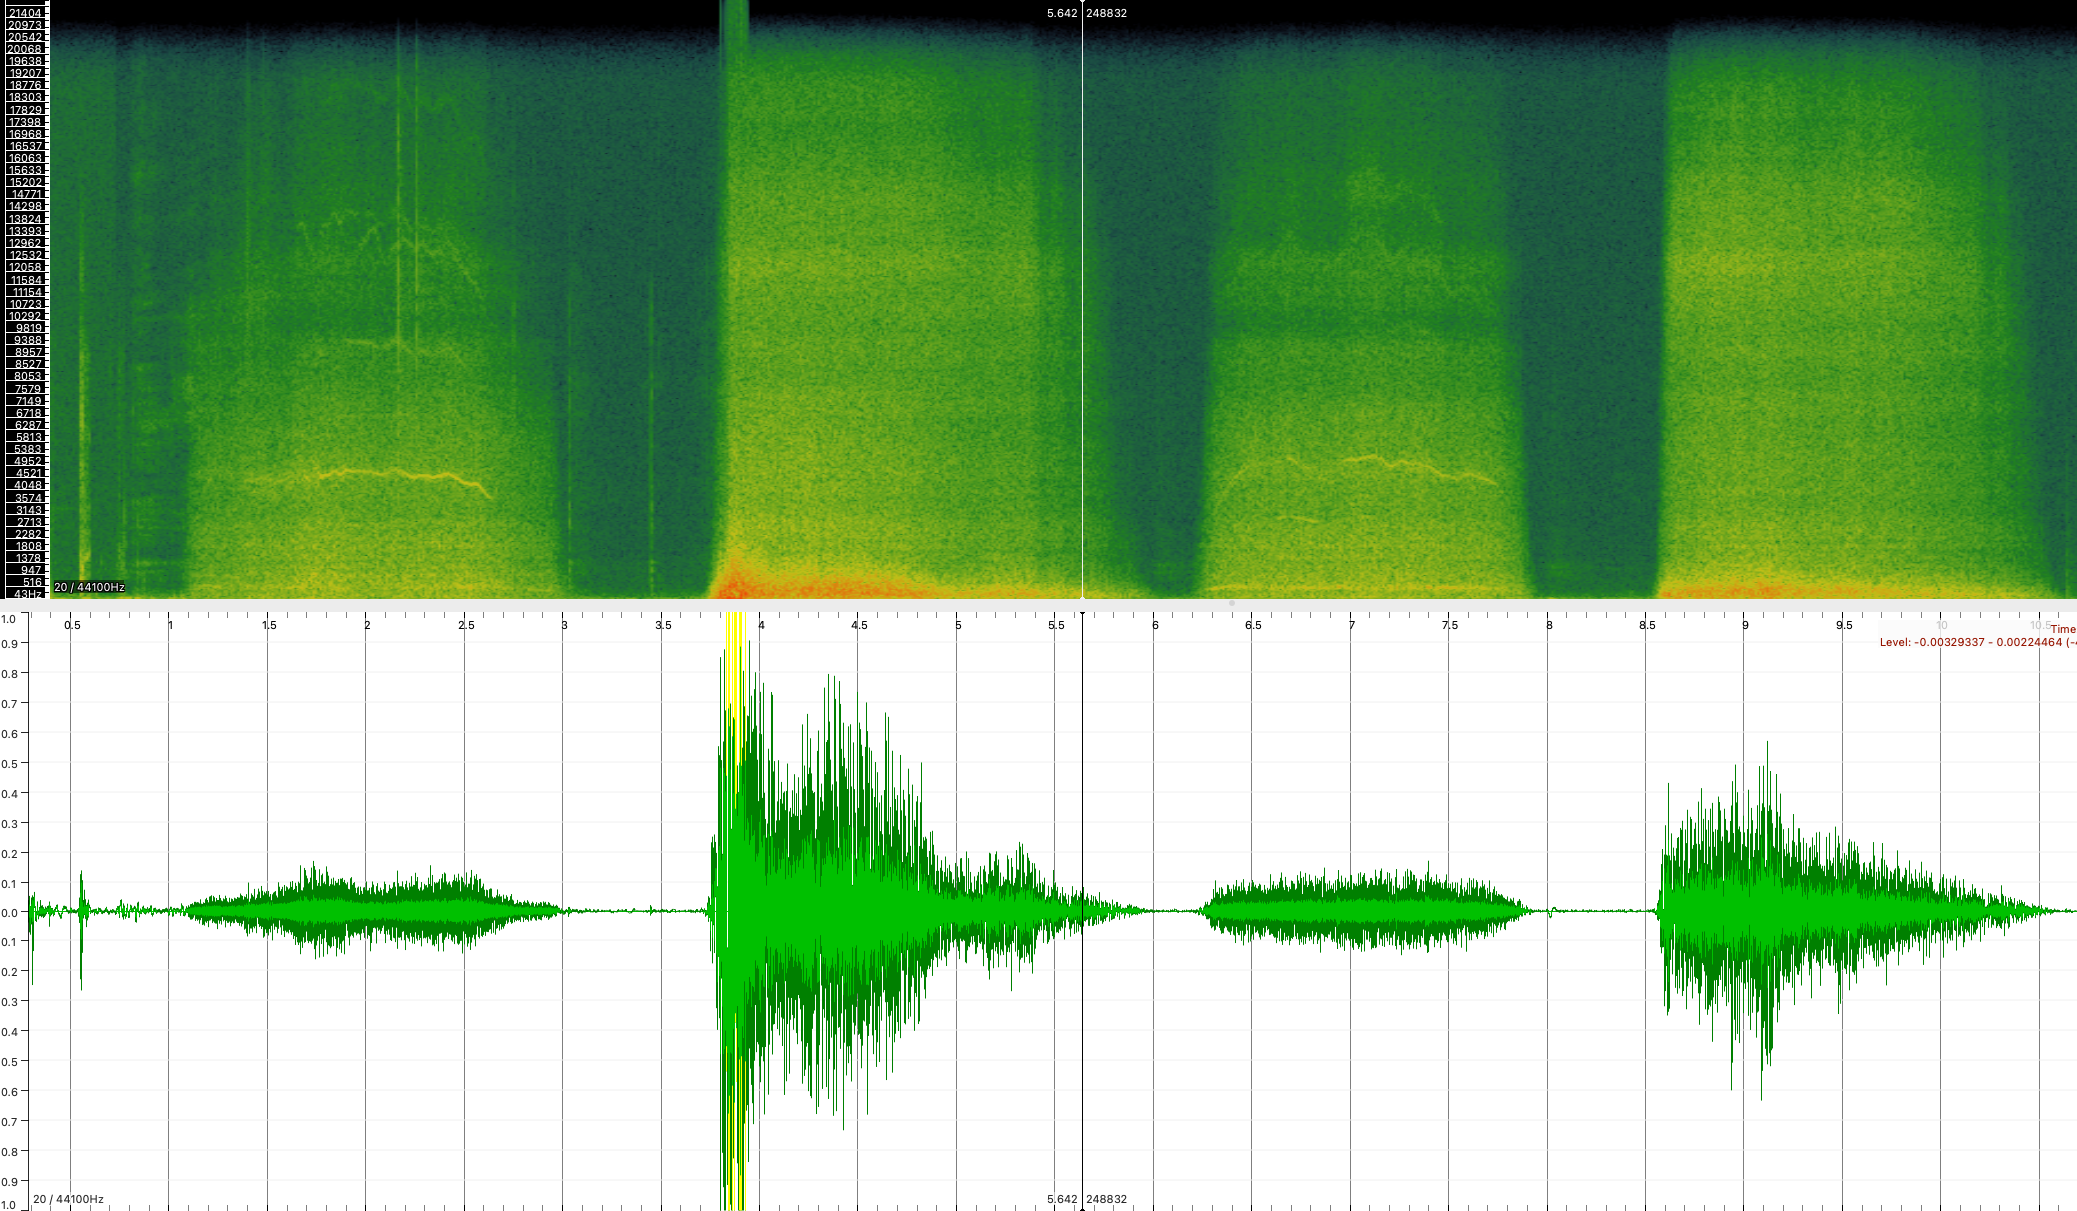
\includegraphics[width=10cm]{stft2}
	\caption{Przykład sygnału wdechu i wydechu nosem poddanego transformacie Fouriera dla okien czasowych - otrzymujemy nowy wymiar informacji, czyli nie tylko natężenie
dźwięku ale też natężenie poszczegółnych częstotliwości w dźwięku. Obraz z programu Sonic Visualizer, który realizuje STFT}
\end{figure}

\subsection{Bramka szumów}
Głowna metoda odszumiana, z której korzystamy to $Spectral$ $Gating$ (rodzaj bramki szumów).  Pierw wyznaczany jest spektrogram sygnału za pomocą $DFT$ i 
tworzony jest próg szumu dla każdej jego częstotliwości.
Częstotliwości progowe służą to stworzenia maski, której potem używamy do usunięcia niechcianych dźwięków.
Następnie ze spektrogramu tworzymy z powrotem natężenie $I(t)$. W projekcie wykorzystujemy gotową implementację bramki szumów z biblioteki $noisereduce$\footnote{\url{https://pypi.org/project/noisereduce/}}. Zdefiniujmy
\begin{gather*}
	SNR = \frac{P_s}{P_n}
\end{gather*}
gdzie $P_n$ - moc szumu, $P_s = P - P_n$ - moc sygnału użytecznego (moc sygnału pomniejszona o moc szumu).
Porównanie przykładowych SNR dla algorytmów usuwania szumu\footnote{Kumar, E. and Surya, K. and Varma, K. and Akash, A. and Kurapati, Nithish Reddy (2023) \emph{Noise Reduction in Audio File Using Spectral Gatting and FFT by Python Modules}}:
\begin{center}
\begin{tabular}{c  | c }
algorytm & SNR \\
\hline
$LMS$ & 2 \\
$Kalman$ & 6 \\
$Spectral$ $Gating$ & 14
\end{tabular}
\end{center}

\subsection{Filtr Savitzky'ego-Golaya}
Filtru Savitzky'ego-Golaya używamy do wygładzenia spektrogramu po przeprowadzeniu DFT.  Polega on na dopasowywaniu zbioru sąsiadujących punktów do wielomianu niskiego stopnia za pomocą metody najmniejszych kwadratów.
Te fragmenty wielomianów są potem łączone w wygładzoną funkcję. Korzystamy z gotowej implementacji
z biblioteki $scipy$. W przypadku sieci neuronowej korzystamy natomiast z warstw konwolucyjnych, nakładających odpowiednie filtry na obraz.
\begin{figure}[H]
	\centering
	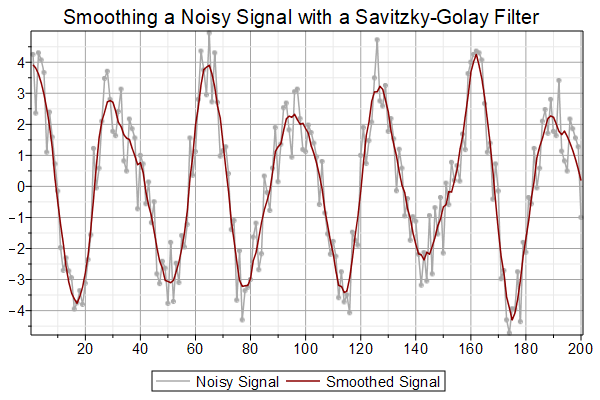
\includegraphics[width=10cm]{savitzky_golay_filter}
	\caption{Wizualizacja działania filtru Savitzky'ego-Golaya dla przykładowego zbioru próbek, \url{https://www.maplesoft.com/Applications/Detail.aspx?id=154593}}
\end{figure}

\subsection{Ocena modeli}
Zastosowaliśmy następujące miary oceny ilościowej modelu:
\begin{flalign*}
	&accuracy = \frac{|TP_{wdech}|+|TN_{wdech}|}{|TP_{wdech}|+|FP_{wdech}|+|TN_{wdech}|+|FN_{wdech}|}&\\
	&precision_{wdech} = \frac{|TP_{wdech}|}{|TP_{wdech}|+|FP_{wdech}|}&\\
	&recall_{wdech} = \frac{|TP_{wdech}|}{|TP_{wdech}|+|FN_{wdech}|}&\\
	&F_{wdech} = \frac{2 \cdot precision_{wdech} \cdot recall_{wdech}}{precision_{wdech} + recall_{wdech}}&
\end{flalign*}
gdzie $TP_{wdech}$ - ilość próbek oznaczonych jako wdech, które sklasyfikowane zostały jako wdech,
$TN_{wdech}$ - ilość próbek nieoznaczonych jako wdech, które nie zostały sklasyfikowane jako wdech,
$FP_{wdech}$ - ilość próbek nieoznaczonych jako wdech, które zostały sklasyfikowane jako wdech,
$FN_{wdech}$ - ilość próbek oznaczonych jako wdech, które nie zostały sklasyfikowane jako wdech.
Analogicznie definiujemy $precision_{wydech}, recall_{wydech}, F_{wydech}$.
\subsection{Standaryzacja}
Dane wejściowe do modelu zawsze standaryzujemy, czyli
\begin{gather*}
	\tilde X = \frac{X - EX}{\sigma_X}
\end{gather*}
stosujemy gotową implementację z biblioteki "scikit-learn" lub warstwę normalizacyjną w przypadku sieci neuronowej.
\subsection{SVM}
Pierwszym modelem, jakim dokonujemy klasyfikacji, jest SVM. Metoda ta polega na szukaniu optymalnych wag $\boldsymbol{w}, b$.
Następnie będziemy klasyfikować według funkcji maszyny uczącej 
\begin{gather*}
	f(x) = sgn(\boldsymbol{w}^T \boldsymbol{x} + b)
\end{gather*}
jeśli $f$ zwraca 1 to traktujemy to jako jedną z binarnych decyzji (w naszym przypadku np. wdech) a jeśli zwraca -1 to drugą (czyli np. wydech).
$\textbf{x}$ jest wektorem cech.  Znalezienie optymalnych wag będzie polegało na minimalizacji
funkcji kosztu
\begin{gather*}
	J(\boldsymbol{w}) = \frac{1}{2}||\boldsymbol{w}||^2 + \frac{C}{N}\Sigma_x max\{0, 1 - y(\boldsymbol{w}^Tx + b)\}
\end{gather*}
gdzie C jest parametrem uregulowania. Funkcję będziemy minimalizować metodą stochastycznego spadku po gradiencie.
W projekcie użyliśmy własnej implementacji SVM-a.
\subsection{Sieć neuronowa}
Drugim modelem jakim dokonujemy klasyfikacji jest sieć neuronowa. Ze względu na trudność w samodzielnym zaprojektowaniu dobrej sieci neuronowej postanowiliśmy użyć "gotowca" a więc stworzonego przez firmę Google Tensorflow'a wraz z interfejsem Keras. \# TODO opisać jak działa ta sieć
\section{Nagrywanie danych oddechowych}
Żeby zapewnić dobre oznaczenie danych, etykietujemy je jeszcze w trakcie nagrywania dźwięku. 
Osoba nagrywana naciska przycisk, żeby zasygnalizować, że przestała brać wdech i zaczyna wydychać 
powietrze lub na odwrót. Momenty przejścia z wdechu na wydech i w drugą stronę zapisywane są w pliku
.csv, a dźwięk w pliku .wav. Częstotliwość próbkowania ustalamy na $44,1$ kHz.
\begin{figure}[H]
	\centering
	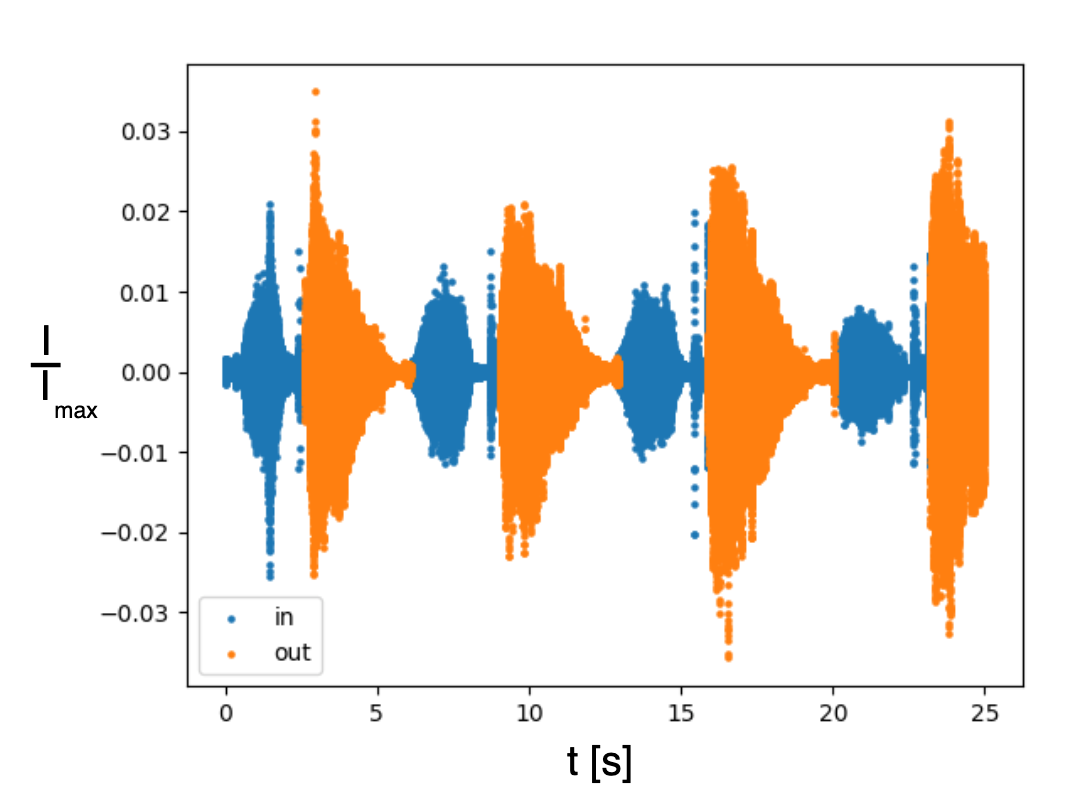
\includegraphics[width=10cm]{nagrywanie_ozn}
	\caption{Przykładowe nagrane dane, in-wdech, out-wydech. Jak widać dane oznaczone na żywo są bardzo dokładne, być może nie bylibyśmy w stanie osiągnąć takiej
dokładności oznaczając ręcznie (lub byłoby to bardzo żmudne).}
\end{figure}
\section{Oddychanie na żywo}
Testowanie modeli do predykcji na żywo odbywało się za pomocą programu wizualizującego aktualnie
stwierdzany stan. 
\begin{figure}[H]
	\centering
	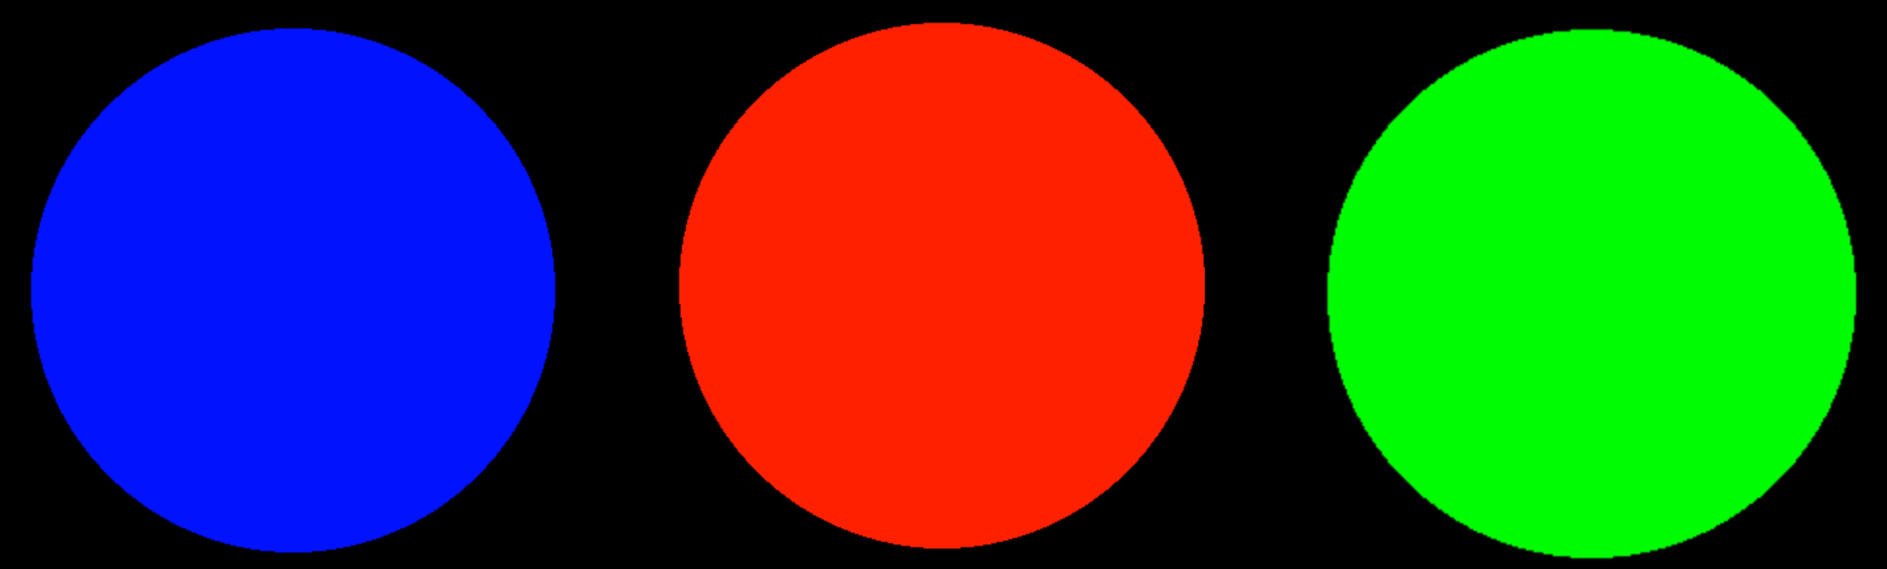
\includegraphics[width=10cm]{wdechwydechcisza}
	\caption{Jeżeli koło zwiększa się i jest niebieskie to model wykrywa wdech, jeśli zmniejsza się i jest
czerwone to jest to wydech, natomiast kolor zielony oznacza, że natężenie dźwięku nie przekracza pewnego 
progu dobieranego eksperymentalnie w zależności od mikrofonu.
Dalej klasyfikacja na żywo nazywana jest też testem jakościowym.}
\end{figure}

\section{Przeliczanie częstotliwości z DFT}
W celu wyznaczenia sposobu zamiany częstotliwości otrzymanej za pomocą DFT na znaną jednostkę (Hz) wykonaliśmy kilkanaście nagrań z ustaloną (w Hz) dominującą częstotliwością i odczytaliśmy, której wartości częstotliwości otrzymanej za pomocą DFT odpowiada maksymalne natężenie. Wyniki przedstawia rysunek 1.
\begin{figure}[H]
	\centering
	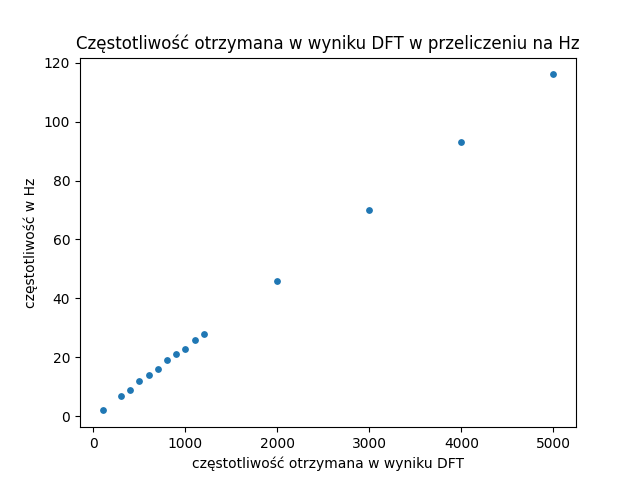
\includegraphics[width=10cm]{przeliczanie_dft_hz}
	\caption{}
\end{figure}
\noindent Po zaobserwowaniu w przybliżeniu liniowego charakteru tej relacji zastosowaliśmy metodę najmniejszych kwadratów do wyznaczenia najlepiej dopasowanej prostej. Otrzymaliśmy następujące wyniki:
\begin{gather*}
	f_{\unit{Hz}}\approx43,0789\,f_{\unit{DFT}}-2,8174,\\
	f_{\unit{DFT}}\approx0,0232\,f_{\unit{Hz}}+0,068,
\end{gather*}
gdzie $f_{\unit{DFT}}$ to wartość liczbowa częstotliwości w jednostkach, w której otrzymuje się wynik DFT, natomiast $f_{\unit{Hz}}$ to wartość liczbowa częstotliwości wyrażonej w \unit{Hz}.
Jeżeli koło zwiększa się i jest niebieskie to model wykrywa wdech, jeśli zmniejsza się i jest
czerwone to jest to wydech, natomiast kolor zielony oznacza, że natężenie dźwięku nie przekracza pewnego 
progu dobieranego eksperymentalnie w zależności od mikrofonu.
Dalej klasyfikacja na żywo nazywana jest też testem jakościowym.
\section{Przyjęty model oddechu}
Na początku przyjmujemy model "sportowego" oddychania, czyli wdech nosem i wydech ustami.
Uproszczenie to polega na tym, że wydawane dźwięki są dosyć różne, dopiero potem sprawdzamy jak nasze podejście będzie się sprawować
przy innych metodach oddychania.
\begin{figure}[H]
	\centering
	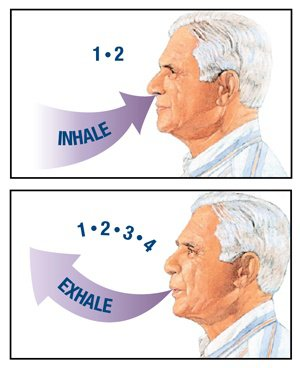
\includegraphics[width=3cm]{model_oddechu}
  	\caption{Ilustracja przyjętego modelu,  \href{https://www.quora.com/Should-I-exhale-from-the-mouth-or-nose-while-deep-breathing}{źródło}}
\end{figure}
\section{Średnia częstotliwość w czasie}
\subsection{Metoda}
Pierwotnie przyjętym założeniem było, że podczas wdechu średnia częstotliwość dźwięku jest wyższa niż
gdy osoba wydycha. Z pliku w formacie .wav pobieramy natężenie, które następnie \textbf{odszumiamy} za pomocą $noisereduce$ (przy testach jakościowych stosujemy bramkę szumów dla 3 ostatnich sekund) . 
\textbf{Dzielimy próbki na bloki, dla których tworzymy spektrogramy} i obliczamy
średnią ważoną częstotliwość.
Cechami, na podstawie których dokonywana jest predykcja są  
\begin{gather*}
\boldsymbol x (t_n) = [\bar{f}(t_0), \bar{f}(t_1), ..., \bar{f}(t_n)]
\end{gather*}
czyli średnie częstotliwości z kilku przeszłych chwil.
Dla danych testowych spełniających powyższe założenie i modelu wytrenowanego SVM-em dawało nam to dokładność $\sim 60\%$.
\begin{figure}[H]
	\centering
	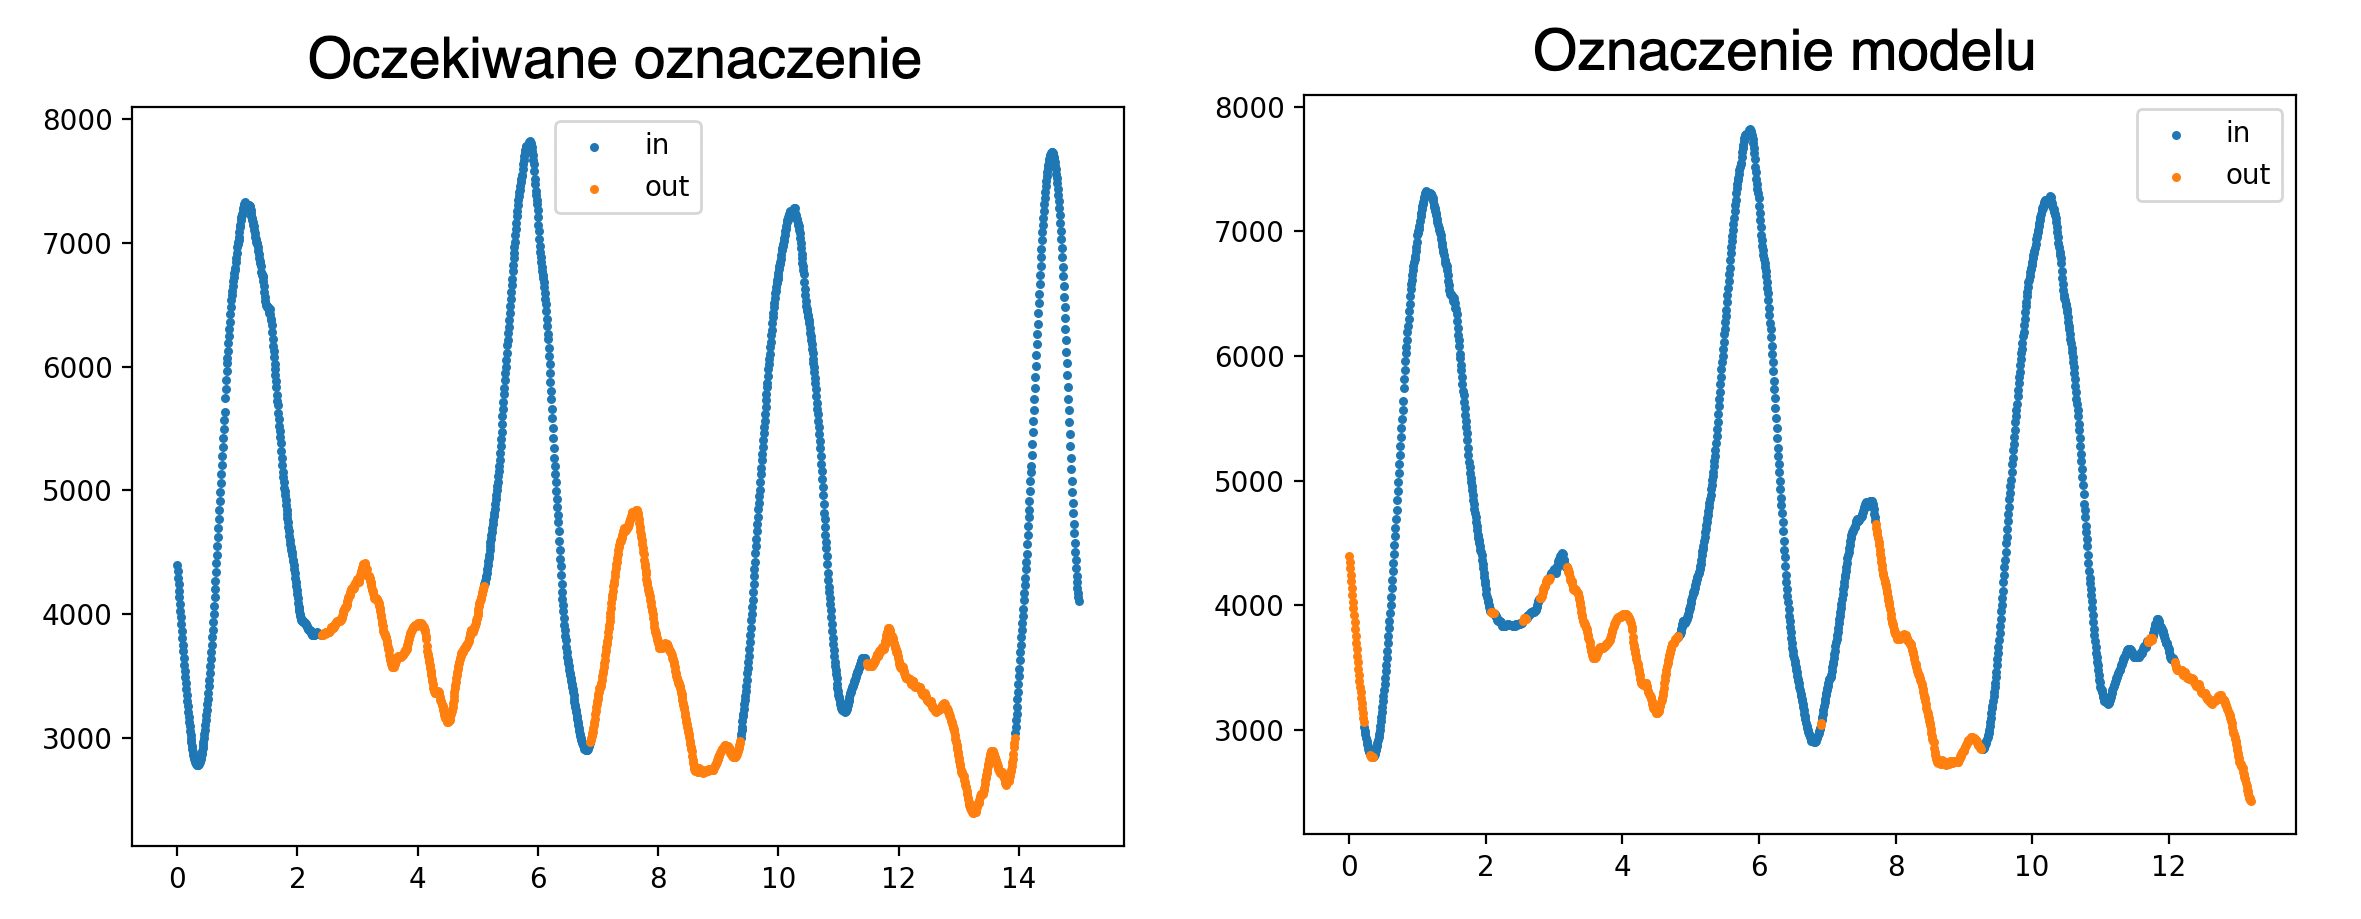
\includegraphics[width=10cm]{porownanie_srednie}
	\caption{Przykładowe działanie modelu dla danych spełniających założenie: wyższy wdech, niższy wydech.
	W pewnych momentach podobnie wyglądające fragmenty krzywej powinny być wdechem, w innych wydechem, mamy więc możliwy underfitting.}
\end{figure}
\subsection{Problemy}
Podejście to jednak mocno ograniczna nasze dalsze pole do rozwoju.  Zmniejszenie całego 
spektrogramu do pojedynczej wartości częstotliwości daje nam mniej informacji, przez co 
być może ograniczylibyśmy się tylko do przyjętego przez nas modelu (tj.  wdech - nos, wydech - usta) - w innych
modelach różnica średnich częstotliwości między wdechem a wydechem może nie być taka wyraźna.  Ponadto, dla niektórych osób zaobserwowaliśmy, 
że zależność między wdechem a wydechem jest niekoniecznie tak prosta jak założyliśmy. Obserwowana metoda
była również bardzo niestabilna jeżeli chodzi o testy jakościowe (klasyfikację na żywo).
\begin{figure}[H]
	\centering
	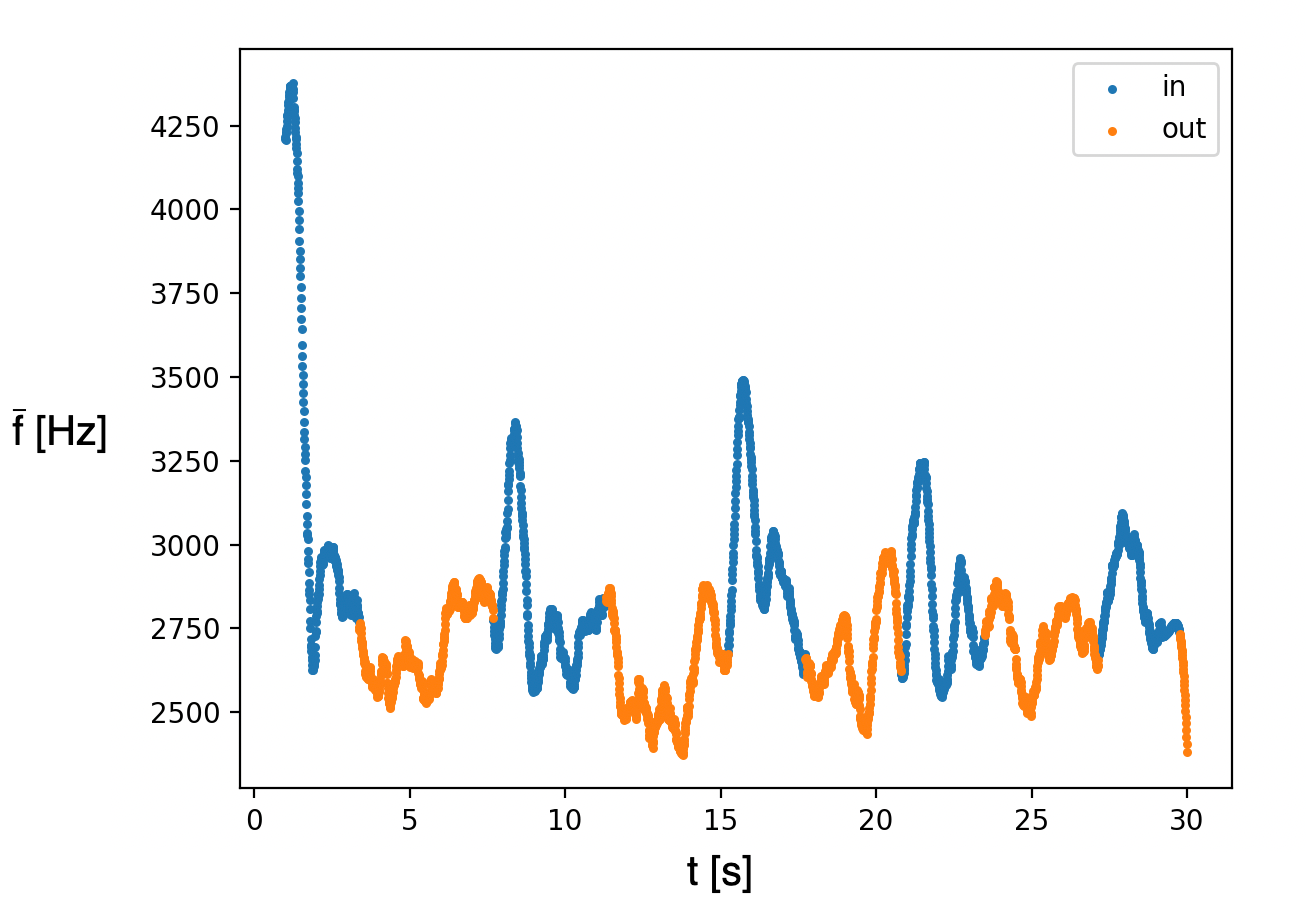
\includegraphics[width=10cm]{problem_srednie_ozn}
	\caption{Nieoczywista zależność między wdechem a wydechem.}
\end{figure}

\section{Dane wejściowe ze spektrogramu + SVM}
\subsection{Założenie}
Kolejnym przyjętym przez nas podejściem było wzięcie całego spektrogramu (a przynajmniej jego części) jako dane wejściowe do SVM-a.  
Metoda pochodzi od przypuszczenia, że człowiek rozpoznaje i rozróżnia wdech/wydech
na podstawie barwy dźwięku.  
\begin{figure}[H]
	\centering
	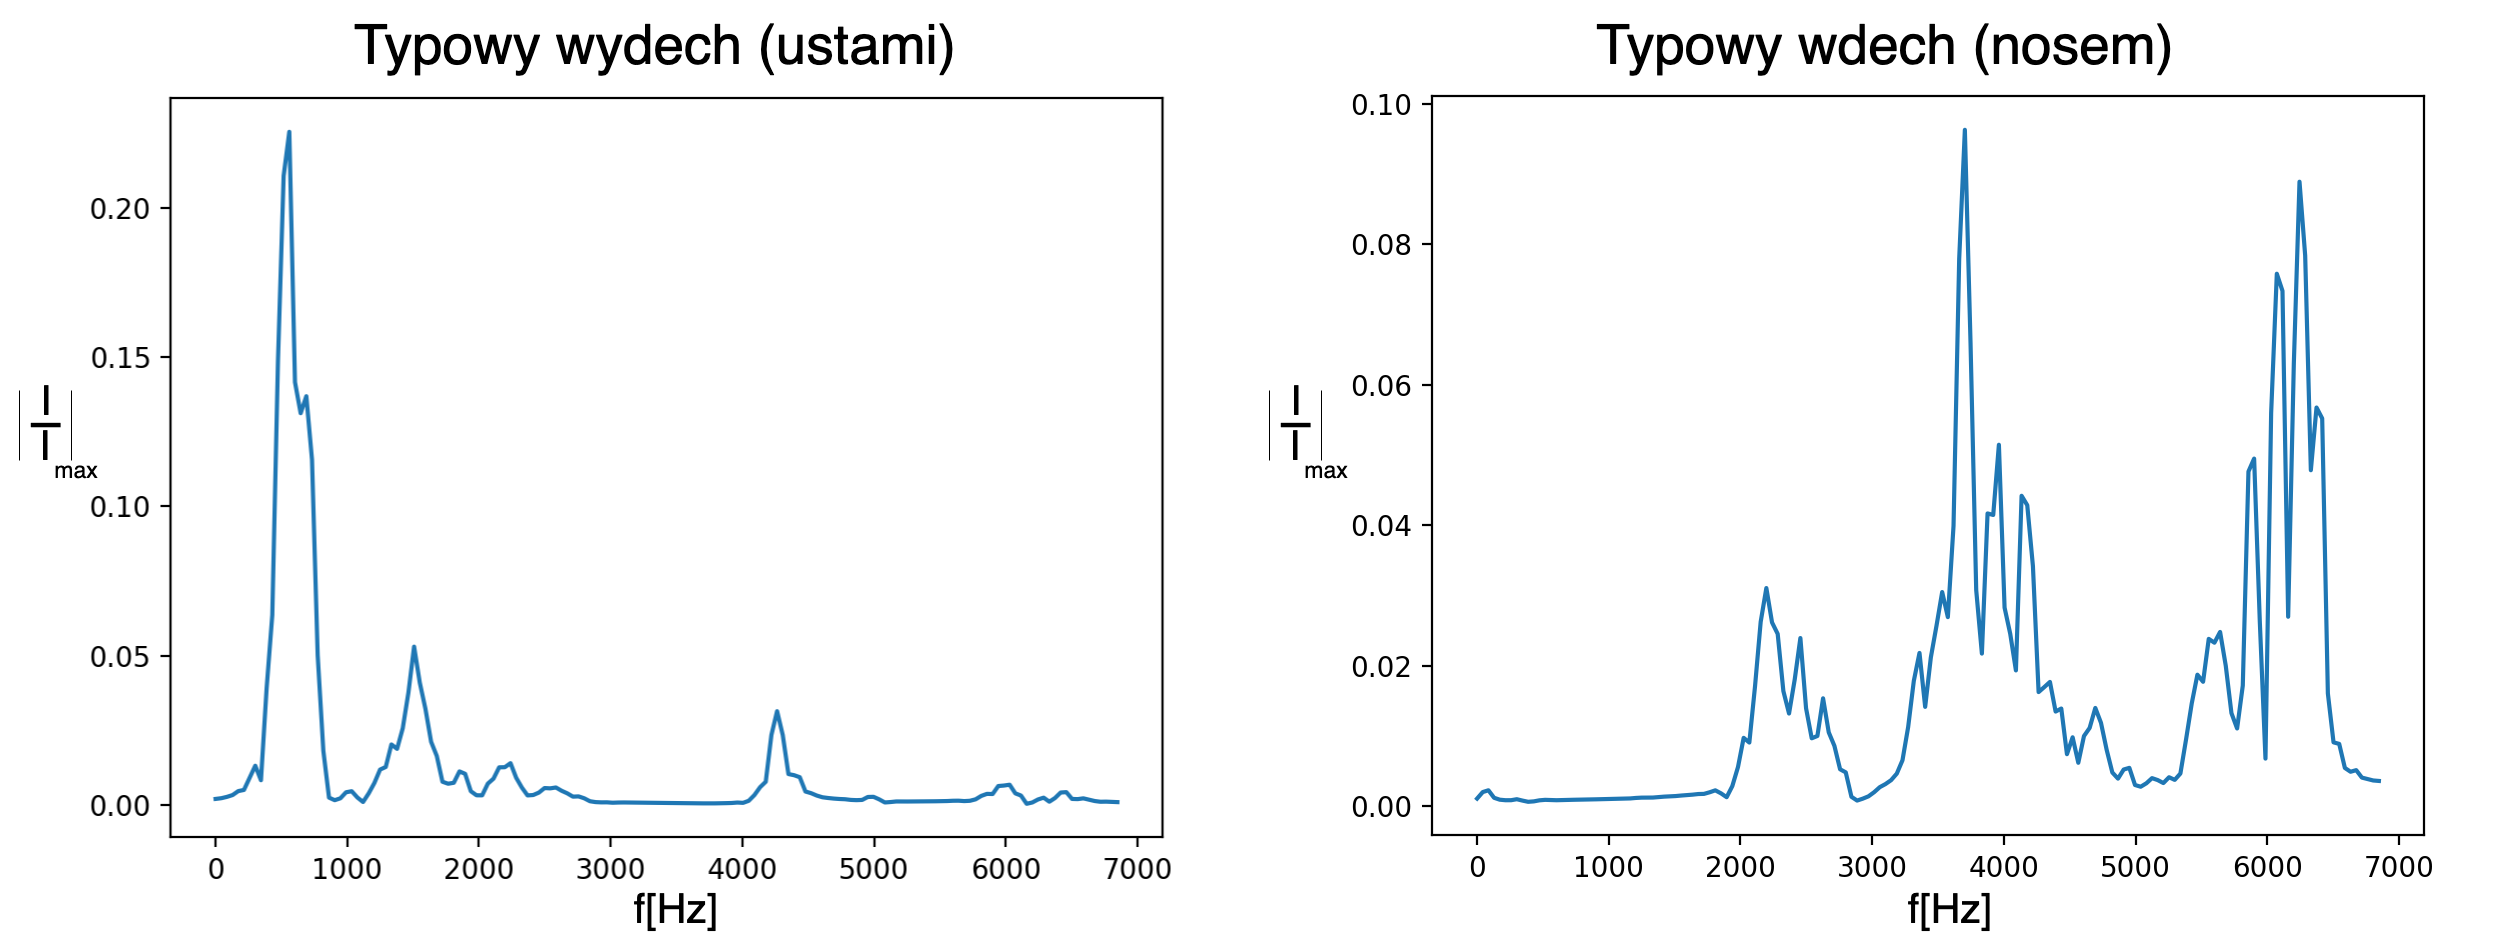
\includegraphics[width=10cm]{wdech_wydech_spektro}
  	\caption{Nie są istotne dokładne kształty powyższych spektrogramów, tylko fakt, że wydech
jest pojedynczym pikiem $\in (0, 1)$ kHz a wdech częstotliwościami z natężeniem
o mniejszym odchyleniu $\in (2, 7)$ kHz.  Zbliżoną zależność zaobserwowano dla paru osób.}.
\end{figure}
\subsection{Metoda}
Podobnie jak ostatnio pierw odszumiamy sygnał z pliku za pomocą $noisereduce$. \textbf{Dzielimy dane na bloki
rozmiaru 1024 próbek, tworzymy dla każdego bloku spektrogram} ale tym razem nie liczymy średniej tylko zostawiamy całą taką klatkę. Wektor cech ma więc postać 
\begin{gather*}
\boldsymbol{x} = [I_{f_1}, I_{f_2}, ..., I_{f_n}]
\end{gather*}
Nie są nam potrzebne wszystkie częstotliwości zwracane przez algorytm DFT, więc stosujemy ograniczenie podobne
do tego stosowanego w telefonii komórkowej -  \textbf{używamy 160 częstotliwości z przedziału do 6,9 kHz}.
Stosując to podejście dla danych testowych otrzymaliśmy następujące wyniki:
\begin{flalign*}
	&accuracy \approx 94\% &\\
	&precision_{wdech} \approx 99\% &\\
	&precision_{wydech} \approx 79\% &\\
	&recall_{wdech} \approx 60\% &\\
	&recall_{wydech} \approx 100\% &\\
	&F_{wdech} \approx 75\% &\\
	&F_{wydech} \approx 88\%. &
\end{flalign*}
W testach jakościowych jednak zaobserwować było można "przeskakiwanie" z jednej
wartości na drugą i z powrotem np. w połowie brania wdechu, wydychania.
\begin{figure}[H]
	\centering
	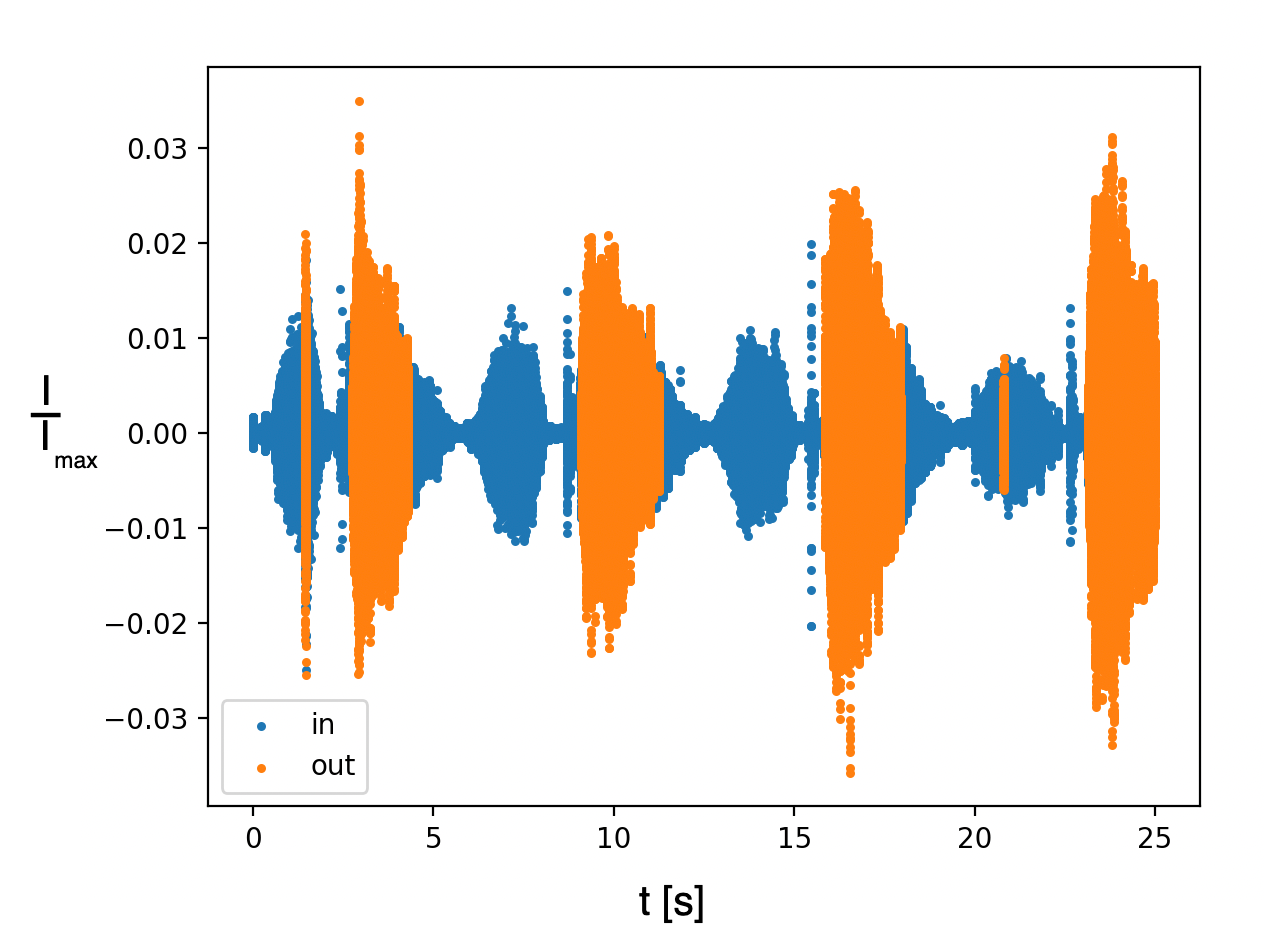
\includegraphics[width=10cm]{przeskakiwanie_ozn}
  	\caption{Dane z rysunku 1. oznaczone, jak widać, występują przeskoki z jednej wartości na drugą.}
\end{figure}

\subsection{Poprzedni stan}
W celu pozbycia się "przeskakiwania" i ogólnej poprawy działania dane z poprzedniego podpunktu rozszerzyliśmy o informację o \textbf{wcześniej przewidzianym stanie}, czyli 
\begin{gather*}
	\boldsymbol{x} = [I_{f_1}, I_{f_2}, ..., I_{f_{160}},  s]
\end{gather*}
 gdzie $s = 1$ jeśli poprzednio stwierdzono wdech, $s=-1$ jeśli poprzednio stwierdzono wydech.
Dodatkowo przeprowadziliśmy jeszcze \textbf{wygładzenie spektrogramu filtrem Savitzky'ego-Golaya}. Następnie przetestowaliśmy program w sposób uproszczony -- jako wartość $s$ stanu poprzedniego stosowaliśmy tę odczytaną z
danych testowych, czyli zakładaliśmy za każdym razem, że nasz model przewidzi dobrze poprzedni stan. Otrzymaliśmy następujące wyniki:
\begin{flalign*}
	&accuracy \approx 99\% &\\
	&precision_{wdech} \approx 99\% &\\
	&precision_{wydech} \approx 99\% &\\
	&recall_{wdech} \approx 99\% &\\
	&recall_{wydech} \approx 99\% &\\
	&F_{wdech} \approx 99\% &\\
	&F_{wydech} \approx 99\%. &
\end{flalign*}
Przypadek ten nie jest realny, ponieważ model nie będzie znał poprawnej poprzedniej klasyfikacji, lecz 
zakładał, że to co sam stwierdził jest poprawne. Odczytując poprzedni stan nie z danych testowych, a z poprzedniej
klasyfikacji modelu, otrzymujemy gorsze, choć bardziej miarodajne wyniki:
\begin{flalign*}
	&accuracy \approx 85\% &\\
	&precision_{wdech} \approx 88\% &\\
	&precision_{wydech} \approx 84\% &\\
	&recall_{wdech} \approx 72\% &\\
	&recall_{wydech} \approx 93\% &\\
	&F_{wdech} \approx 79\% &\\
	&F_{wydech} \approx 88\%. &
\end{flalign*}
Wniosek z tego jest taki, że model
z wysokim prawdopodobieństwem przewidzi dobrze kolejny stan, jeżeli dobrze przewidział poprzedni. 
Warto dodać, że rzeczywiście metoda z poprzednim stanem pozwoliła nam ograniczyć "przeskakiwanie" 
w testach jakościowych.
\subsection{Problemy}
W poprzednim podpunkcie wyszedł główny mankament tej metody - konieczność założenia, że poprzednio
przewidziany stan jest dobry co nie zawsze jest prawdą. W testach jakościowych zaobserwować można było
"wariowanie" modelu, czyli sekwencję źle przewidzianych stanów.
\subsection{Szerszy spektrogram}
W celu poprawy działania modelu postanowiliśmy dokładniej przeanalizować, które częstotliwości są kluczowe dla poprawnej oceny fazy oddechu. W oparciu o obserwację spektrogramów wybraliśmy kilka możliwych zakresów, w których różnice między wdechem i wydechem są dobrze widoczne:
\begin{itemize}
	\setlength\itemsep{-0.25em}
	\item[--] 0--1\,300 \unit{Hz} i 3\,400--22\,000 \unit{Hz},
	\item[--] 0--14\,000 \unit{Hz},
	\item[--] 0--1\,300 \unit{Hz} i 3\,400--14\,000 \unit{Hz},
	\item[--] 0--8\,500 \unit{Hz} i 10\,000--14\,000 \unit{Hz},
	\item[--] 0--16\,000 \unit{Hz},
	\item[--] 0--1\,300 \unit{Hz} i 3\,400--16\,000 \unit{Hz},
	\item[--] 0--1\,300 \unit{Hz}, 3\,400--8\,500 \unit{Hz} i 10\,000 \unit{Hz}--16\,000 \unit{Hz},
	\item[--] 0--8\,500 \unit{Hz} i 10\,000--16\,000 \unit{Hz}.
\end{itemize}
\begin{figure}[H]
	\centering
	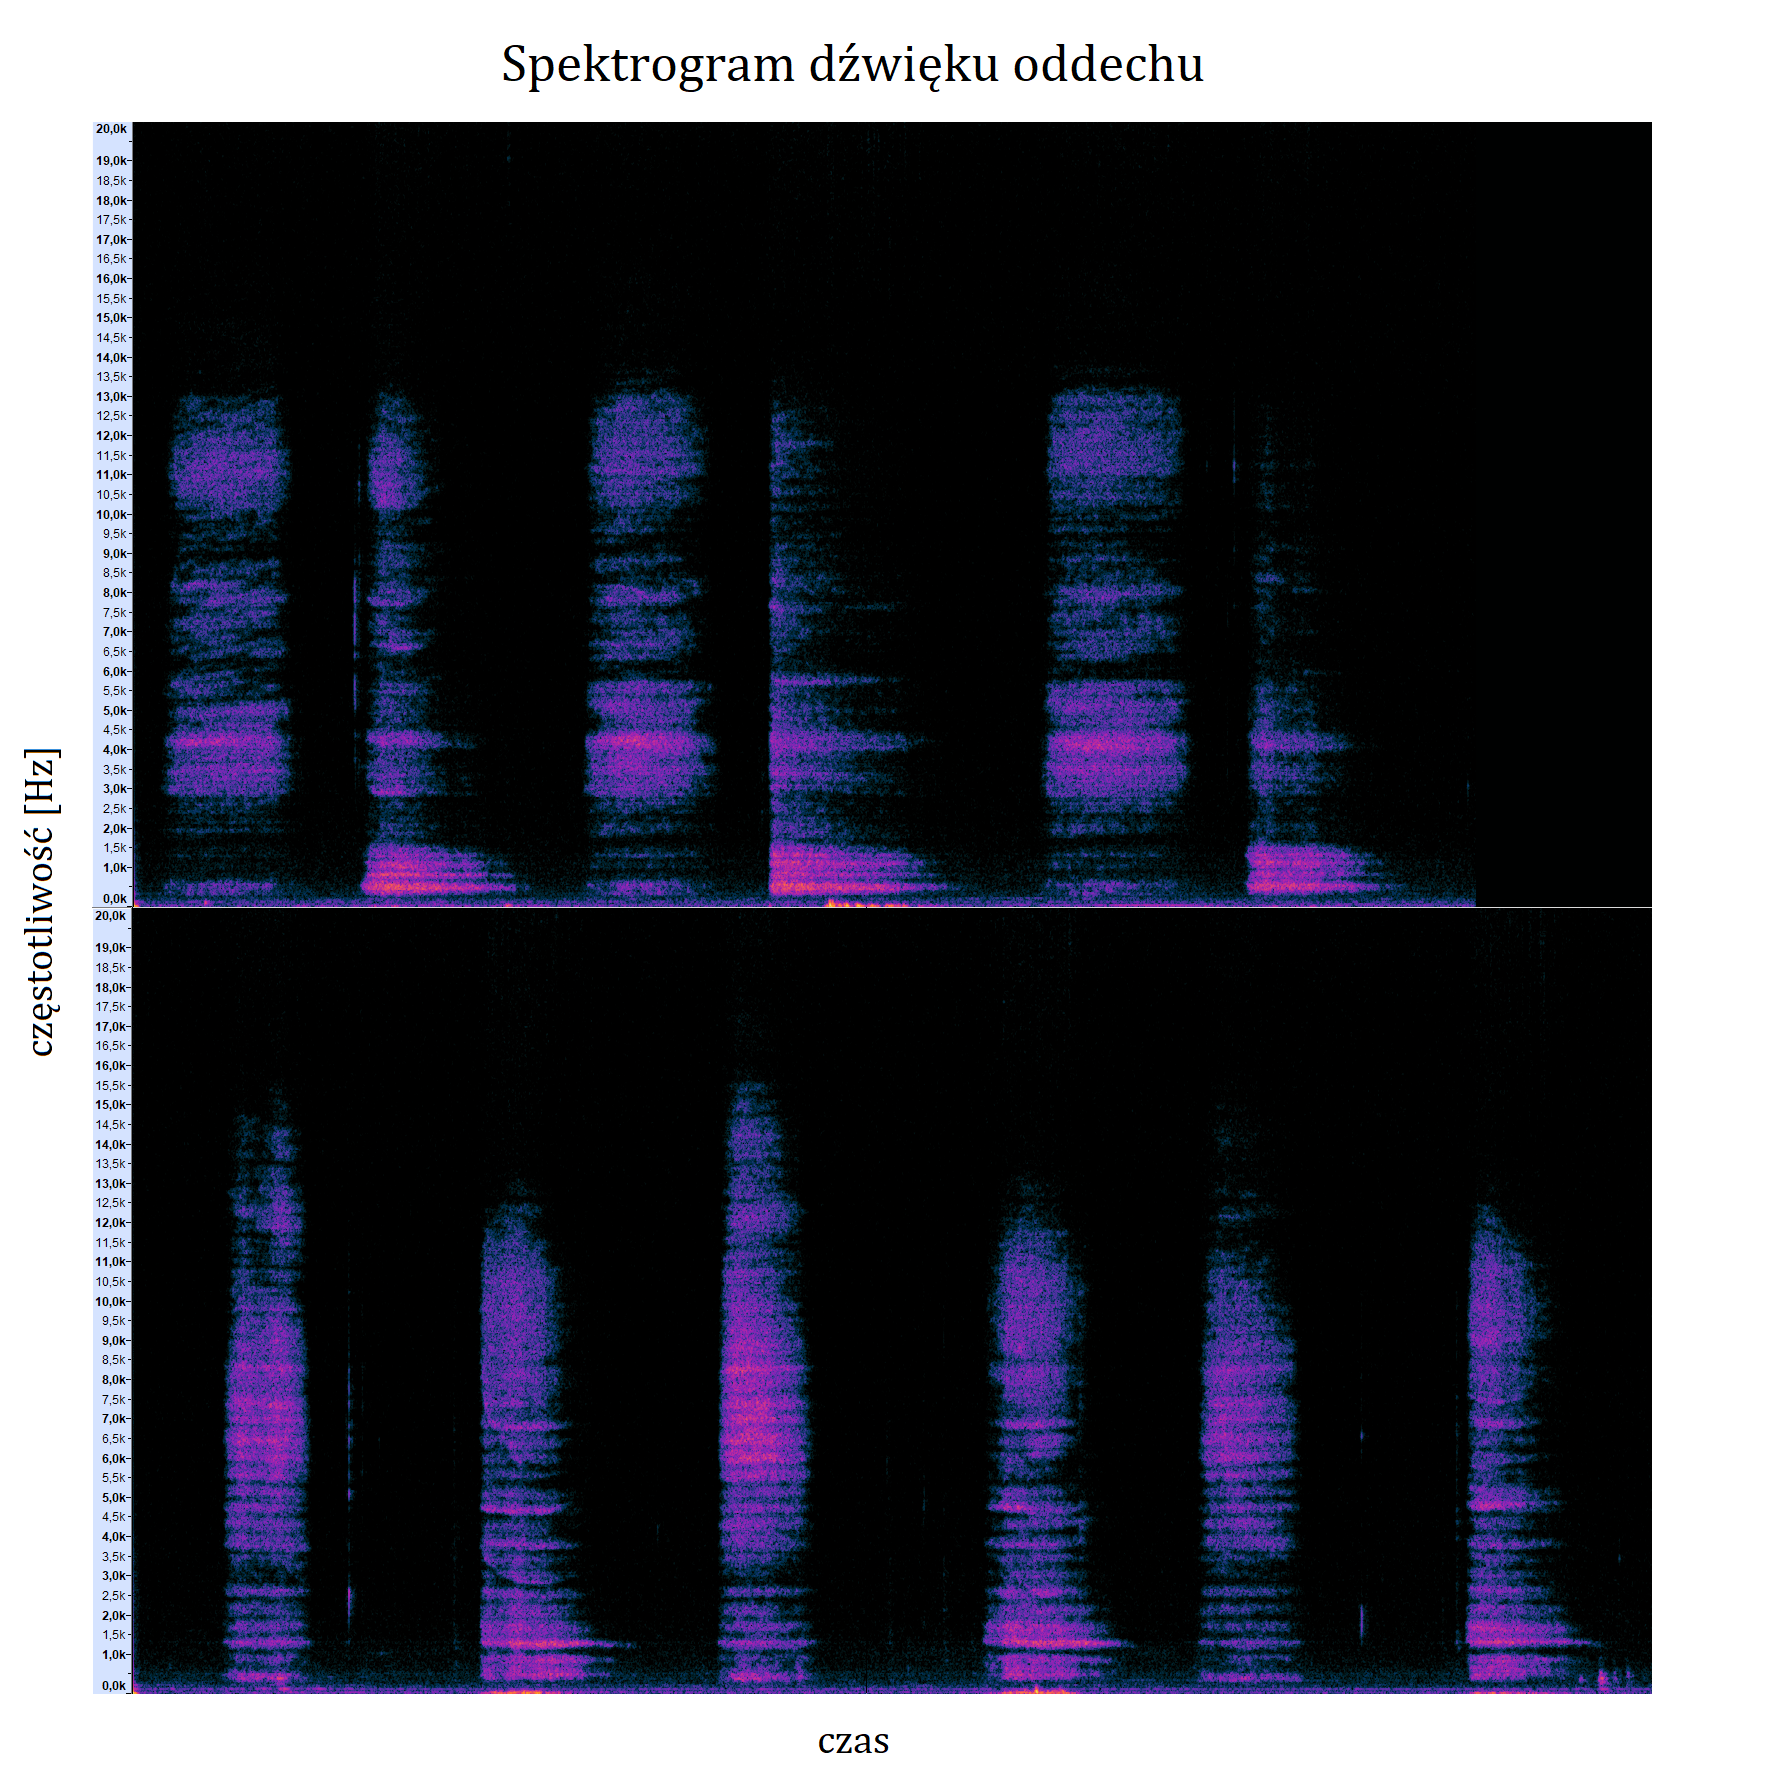
\includegraphics[width=13cm]{spektrogram_wydech_ustami}
	\caption{Spektrogramy dwóch nagrań oddechu z wdechem nosem i wydechem ustami uzyskane przy użyciu programu Audacity.}
\end{figure}
Dla każdego wyboru przeprowadziliśmy testy. W przypadku ostatniego uzyskaliśmy względny wzrost dokładności predykcji o $\sim8\%$ względem początkowego podejścia. Taki wybór częstotliwości przyjęliśmy zatem dla modelu rozpoznającego wdech nosem i wydech ustami.

\section{Dane wejściowe z mikrofonu + Sieć neuronowa}
\subsection{Założenie}
Do przetestowania działania sieci neuronowej przyjęliśmy nieco odmienne podejście. Jako dane wejściowe przyjmujemy (podobnie jak w przypadku SVM) spektrogram jednak w tym przypadku stworzony przy użyciu STFT. Dzięki temu model bierze pod uwagę także zmianę widma w czasie.
\subsection{Metoda}
Stosując poszczególne warstwy nasz spektrogram jest odpowiednio przetwarzany tak aby uwidocznić istotne cechy. Wykorzystywane przez nas warstwy (wraz z parametrami) to:
\begin{enumerate}
  \item\texttt{Input} - Punkt wejścia do sieci neuronowej
  \item\texttt{Resizing} - Zmiana rozmiaru obrazu (32x32)
  \item\texttt{Normalization} - Normalizacja cech
  \item\texttt{Conv2D} - Nałożenie odpowiedniego filtru o rozmiarze n x m (lub n x n) na obraz tak aby uwydatnić jego cechy (32, 3, 'relu'). Wykorzystuje funkcję aktywacji.
  \item\texttt{Conv2D} - Tak jak wyżej (64, 3, 'relu')
  \item\texttt{MaxPooling2D} - Downsampling czyli wybranie maksymalnej wartości spośród okna o zadanych wymiarach (2x2)
  \item\texttt{Dropout} - Ustawienie losowych wejść na 0 z częstotliwością n, przeskalowanie pozostałych cech przez 
  $\frac{1}{1-n}$, pozwala na zredukowanie overfittingu (0.25)
  \item\texttt{Flatten} - Spłaszczenie wejścia do 1 wymiaru
  \item\texttt{Dense} - Łączy wszystkie neurony z warstwy poprzedniej ze wszystkimi z warstwy kolejnej, identyfikuje do jakiej klasy przynależy obiekt wejściowy. Wykorzystuje funkcję aktywacji. (128, 'relu')
  \item\texttt{Dropout} - Tak jak wyżej (0.5)
  \item\texttt{Dense} - Tak jak wyżej (2)
\end{enumerate}

\subsection{Wykorzystywane próbki}
W przeciwieństwie do SVM, aktualną predykcję określamy nie na podstawie poprzedniego stanu, lecz dla stanu sprzed pewnej chwili czasowej. W naszym przypadku aktualnie wyświetlany stan pochodzi sprzed około 0,5 s. Oczywiście powoduje to pewne opóźnienie, jednak praktycznie niezauważalne przez użytkownika. Podejście to nie ulega jednak propagacji błędów, którą widzimy w przypadku SVM.
\subsection{Problemy}
Przy rozpoznawaniu próbki zakładamy przynależność do jednej z dwóch klas. W przypadku gdy jako dane wejściowe mamy jedynie wdechy i wydechy nie stanowi to problemu. Gdy jednak chcemy rozpoznać brak oddychania musimy założyć pewien próg pewności co otrzymanej klasyfikacji. Eksperymentalnie przyjęliśmy iż wdech jest wdechem gdy pewność sieci neuronowej wynosi 99\% natomiast co do wydechów przyjęliśmy pewność na poziomie 70\%. 

\section{Przejście na inny model oddychania}
\subsection{Wydech nosem}
Kolejnym krokiem było przeniesienie wypracowanej metody uczenia na rozpoznawanie wdechu oraz wydechu nosem. W takim przypadku różnice między fazami oddechu są mniej zauważalne, co wymagało kolejnych udoskonaleń.
\subsection{Szerszy spektrogram}
Ponownie dokonaliśmy obserwacji spektrogramów, tym razem wyznaczonych dla wdechów i wydechów nosem. Zauważyliśmy kilka zakresów, w których różnice między fazami oddechu są zauważalne:
\begin{itemize}
	\setlength\itemsep{-0.25em}
	\item[--] 0--8\,500 \unit{Hz} i 10\,000--16\,000 \unit{Hz},
	\item[--] 0--3\,000 \unit{Hz} i 6\,000--16\,000 \unit{Hz},
	\item[--] 0--16\,000 \unit{Hz}.
\end{itemize}
\begin{figure}[H]
	\centering
	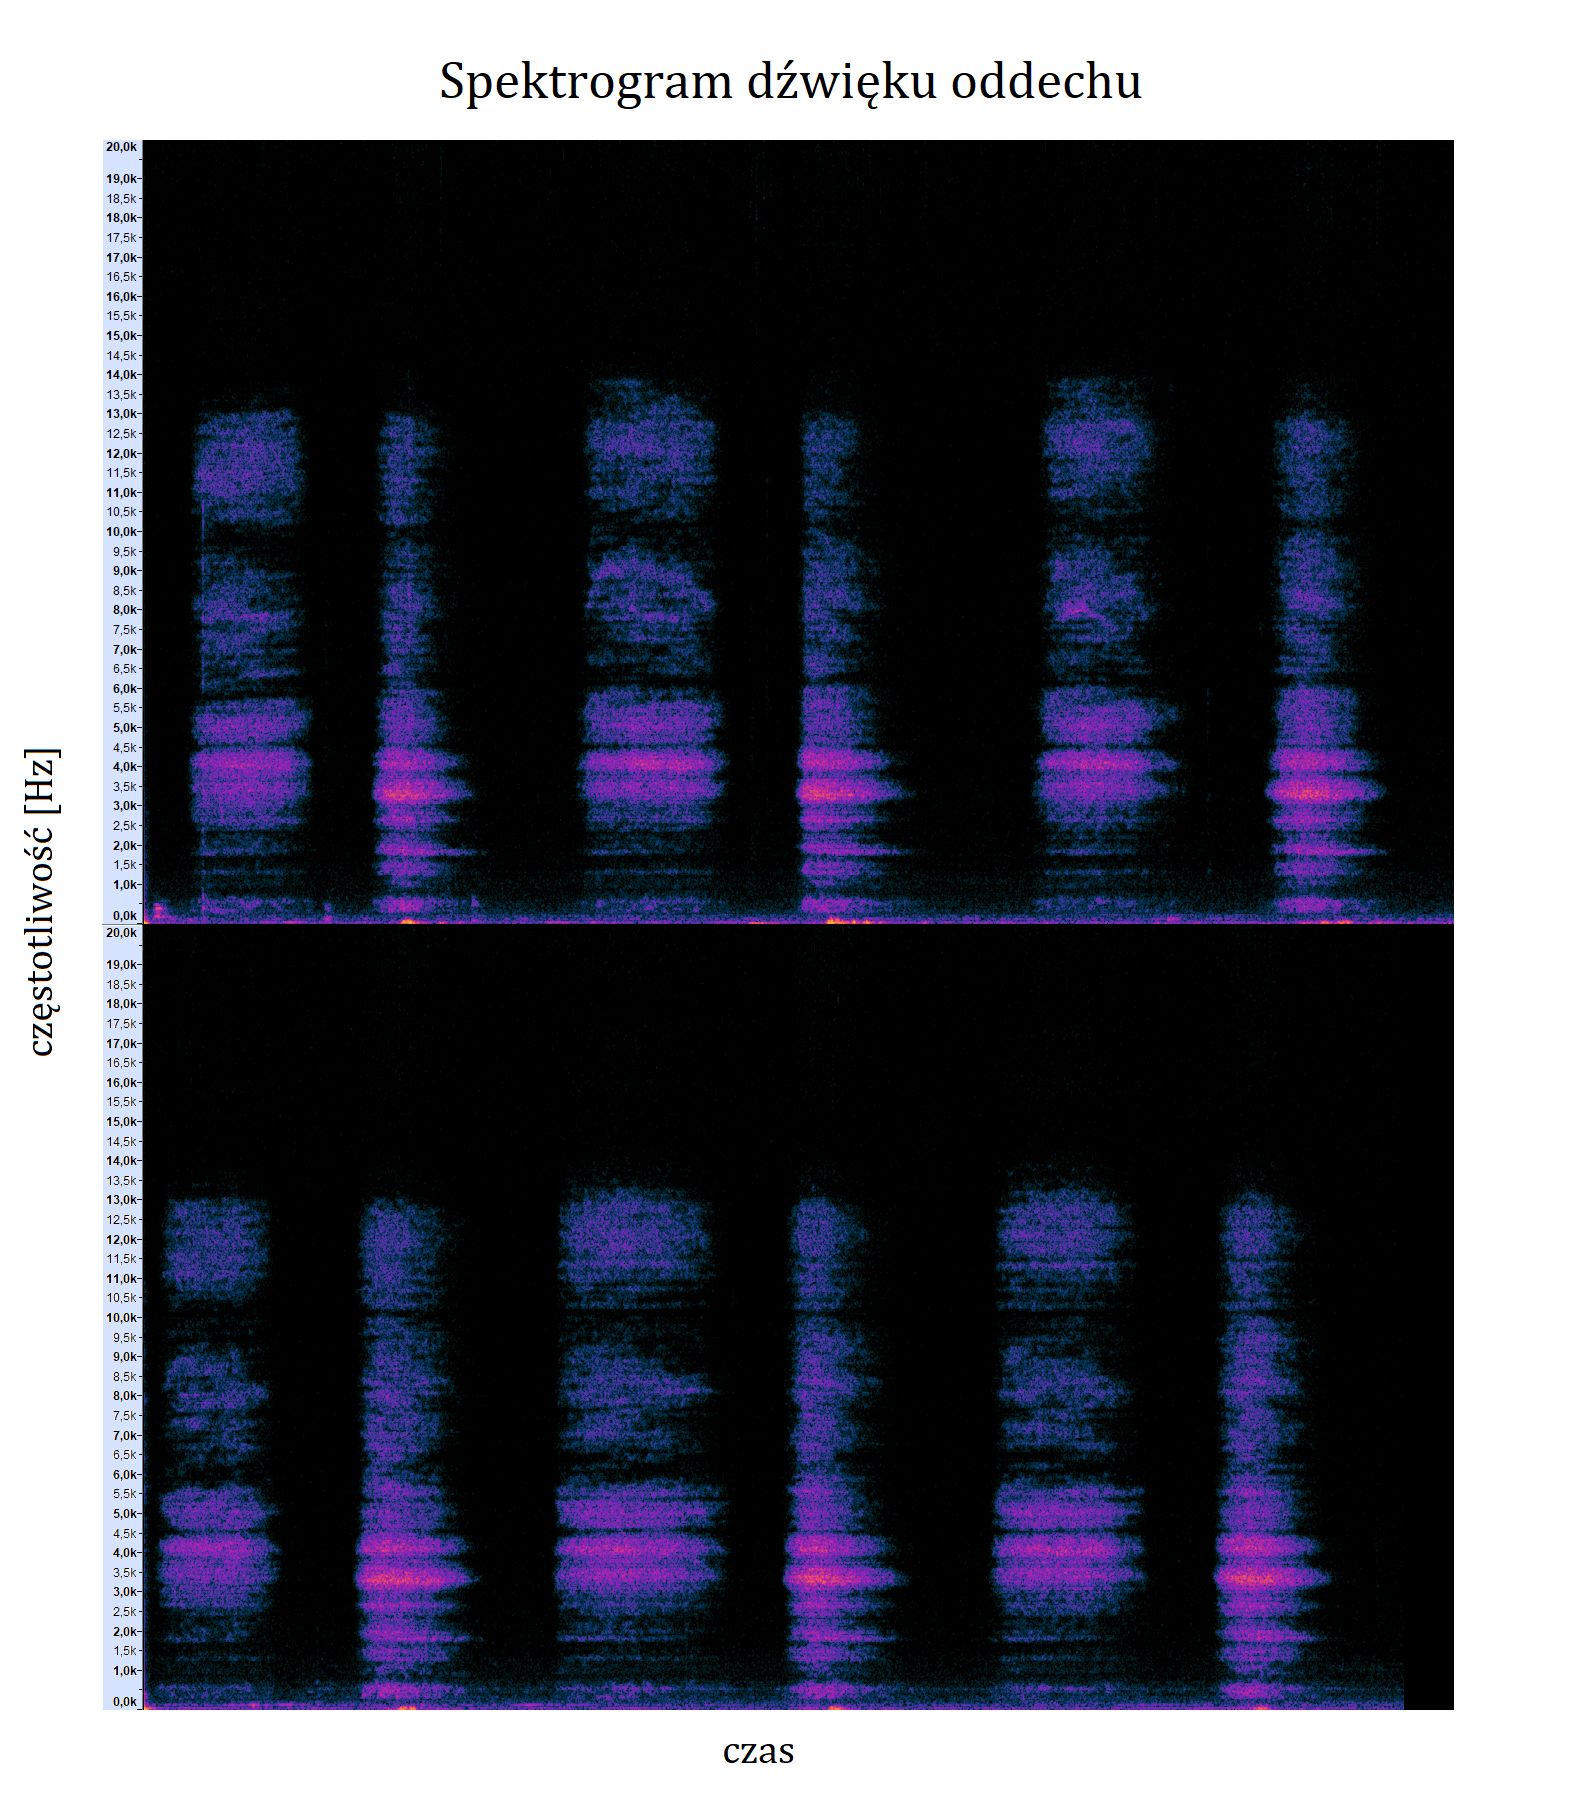
\includegraphics[width=13cm]{spektrogram_wydech_nosem}
	\caption{Spektrogramy dwóch nagrań oddechu z wdechem i wydechem nosem uzyskane przy użyciu program Audacity.}
\end{figure}
Testy pokazały, iż ostatni z powyższych wybór częstotliwości spowodował względny wzrost dokładności o kolejne $\sim7\%$. Taki zatem pozostawiliśmy do dalszej pracy.
\subsection{Usuwanie ciszy}
Nietrudno było zaobserwować, iż znaczą część nagrań zajmuje cisza lub dźwięk bliski ciszy.
\begin{figure}[H]
	\centering
	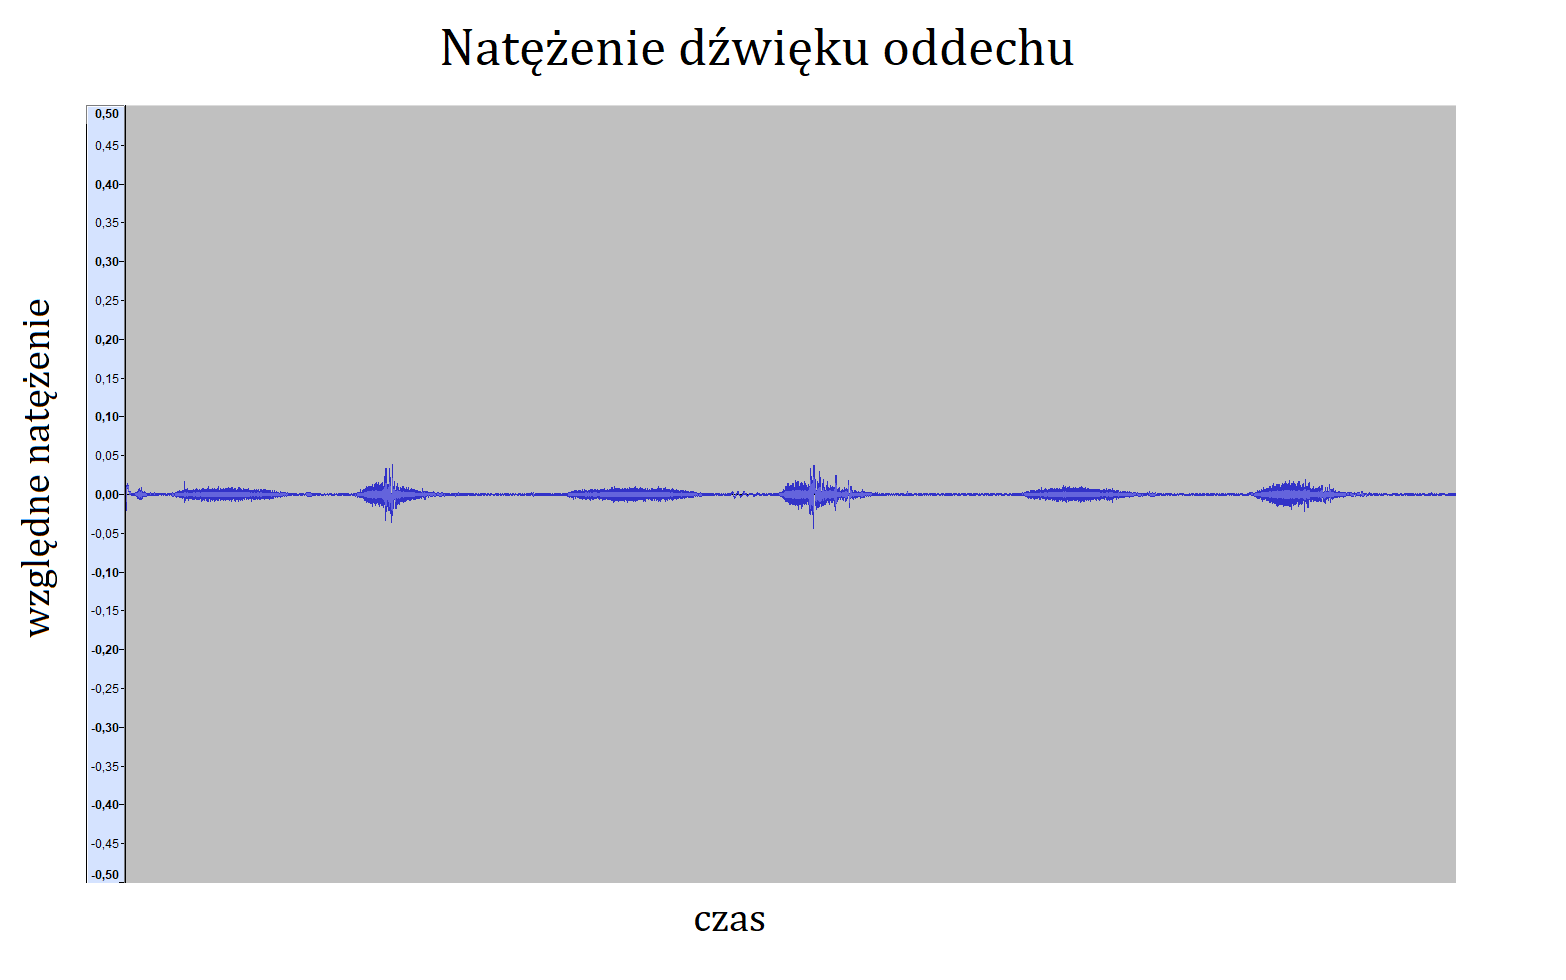
\includegraphics[width=13cm]{natezenie_wydech_nosem}
	\caption{Wykres natężenia dźwięku w nagraniu wdechu i wydechu nosem uzyskany przy użyciu programu Audacity.}
\end{figure}
Te przerwy między wyraźnymi dźwiękami oddechów pozostawały jednak oznaczone jako wdech lub wydech. Z tego powodu model trenowaliśmy w jednym przypadku informacją, iż cisza występuje podczas wdechu, a w innym -- że w trakcie wydechu. Postanowiliśmy usunąć tę niedoskonałość z przypuszczeniem, iż poprawi to wyniki działania programu.

\section{Wnioski}
Todo
\section{Źródła}
\begin{thebibliography}{2}
\bibitem{Cormen} 
 Cormen Thomas H., Leiserson Charles E., Rivest Roland L., Stein Clifford (1989) \emph{Wprowadzenie do algorytmów},
\bibitem{DFT}
\url{https://pl.wikipedia.org/wiki/Dyskretna_transformata_Fouriera}
\bibitem{STFT}
\url{https://esezam.okno.pw.edu.pl/mod/book/view.php?id=9&chapterid=77}
\bibitem{Bramkaszumow}
Kumar, E. and Surya, K. and Varma, K. and Akash, A. and Kurapati, Nithish Reddy (2023) \emph{Noise Reduction in Audio File Using Spectral Gatting and FFT by Python Modules}
\bibitem{SavgolImage}
\url{https://www.maplesoft.com/Applications/Detail.aspx?id=154593}
\bibitem{Głębokie uczenie maszyn}
\url{https://www.deltami.edu.pl/temat/informatyka/sztuczna_inteligencja/2017/12/28/Glebokie_uczenie_maszyn/}
\bibitem{Warstwa w pełni połączona}
\url{http://sciagaprogramisty.blogspot.com/2018/03/fully-connected-layer-fc-warstwa-w-peni.html}
\bibitem{Keras Tutorial}
\url{https://www.tutorialspoint.com/keras}
\end{thebibliography}


\end{document}
